\section{Yêu cầu về hệ thống}

% Định nghĩa kiểu cột mới với căn trái (tránh justify làm chữ thưa)
\newcolumntype{L}[1]{>{\raggedright\arraybackslash}p{#1}}

Phần này trình bày các yêu cầu chức năng và phi chức năng của hệ thống robot trợ lý ảo hỗ trợ chăm sóc và giám sát người cao tuổi tại nhà. Các yêu cầu được phân loại và đặc tả chi tiết dựa trên kiến trúc ba khối chính của hệ thống: Khối Robot tại nhà, Hạ tầng Cloud trung gian, và Khối điều khiển Robot từ xa.

\subsection{Tổng quan kiến trúc hệ thống}

Hệ thống được thiết kế theo kiến trúc phân tán, bao gồm ba thành phần chính:
\begin{figure}[h!]
    \centering
    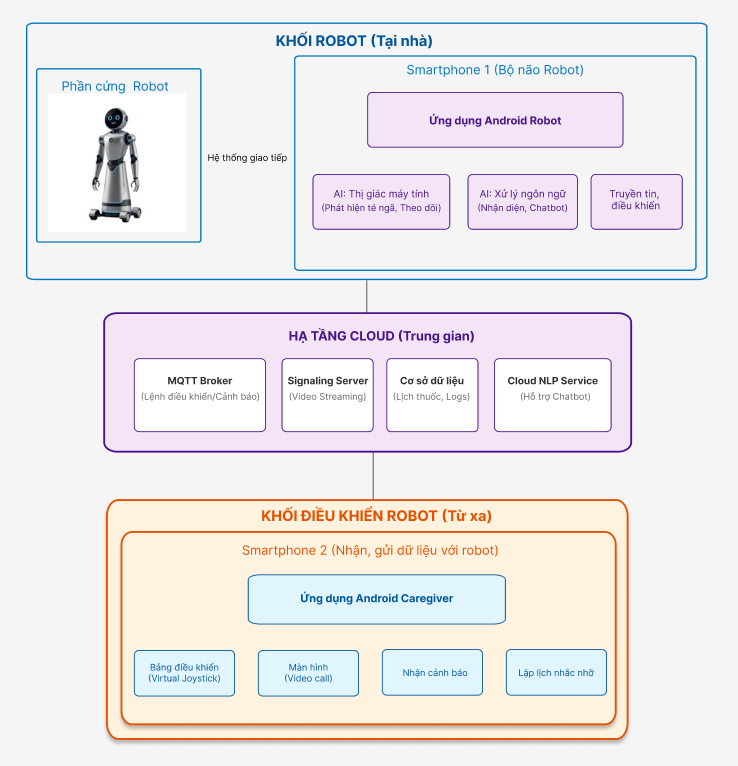
\includegraphics[width=0.95\textwidth]{Images/sơ đồ hệ thống.jpg}
    \vspace{8pt}
    \caption{Sơ đồ kiến trúc tổng thể hệ thống Robot trợ lý ảo}
    \label{fig:system-architecture}
\end{figure}

\begin{itemize}
    \item \textbf{Khối Robot (Tại nhà):} Bao gồm phần cứng robot và smartphone đóng vai trò là bộ não xử lý. Smartphone chạy ứng dụng Android Robot với các module AI: Thị giác máy tính (phát hiện té ngã, theo dõi người) và Xử lý ngôn ngữ (nhận diện giọng nói, chatbot).
    
    \item \textbf{Hạ tầng Cloud (Trung gian):} Đóng vai trò trung gian kết nối, bao gồm MQTT Broker (gửi lệnh điều khiển/cảnh báo), Signaling Server (hỗ trợ video streaming), Cơ sở dữ liệu (lưu trữ lịch thuốc, logs), và Cloud NLP Service (hỗ trợ chatbot).
    
    \item \textbf{Khối Điều khiển Robot (Từ xa):} Smartphone của người chăm sóc với ứng dụng Android Caregiver, cho phép điều khiển robot, xem video call, nhận cảnh báo và lập lịch nhắc nhở.
\end{itemize}

\subsection{Yêu cầu chức năng}
\subsubsection{Nhóm chức năng Giao tiếp bằng Giọng nói (Voice Interaction)}

\begin{table}[h!]
\centering
\label{tab:req-voice}
\begin{tabular}{|L{1.5cm}|L{3.5cm}|L{8.5cm}|}
\hline
\textbf{Mã} & \textbf{Tên yêu cầu} & \textbf{Mô tả chi tiết} \\
\hline
FR-V01 & Nhận dạng giọng nói (STT) & Hệ thống phải có khả năng chuyển đổi giọng nói của người dùng thành văn bản với độ chính xác cao, hỗ trợ tiếng Việt với các giọng vùng miền khác nhau. \\
\hline
FR-V02 & Phát hiện wake word & Robot phải phản hồi khi người dùng gọi từ khóa kích hoạt như ``Robot ơi'' hoặc tên tùy chỉnh. \\
\hline
FR-V03 & Hiểu ngôn ngữ tự nhiên (NLU) & Hệ thống phải có khả năng phân tích ý định (intent) và trích xuất thực thể (entity) từ câu nói của người dùng. \\
\hline
FR-V04 & Tổng hợp giọng nói (TTS) & Robot phải có khả năng phản hồi bằng giọng nói tiếng Việt tự nhiên, dễ nghe và phù hợp với người cao tuổi. \\
\hline
FR-V05 & Hội thoại thông minh & Tích hợp AI Agent (LLM) để duy trì cuộc hội thoại có ngữ cảnh, trả lời câu hỏi và thực hiện các tác vụ theo yêu cầu. \\
\hline
\end{tabular}
\end{table}

\newpage
\subsubsection{Nhóm chức năng Phát hiện và Cảnh báo Té ngã (Fall Detection)}

\begin{table}[h!]
\centering
\label{tab:req-fall}
\begin{tabular}{|L{1.5cm}|L{3.5cm}|L{8.5cm}|}
\hline
\textbf{Mã} & \textbf{Tên yêu cầu} & \textbf{Mô tả chi tiết} \\
\hline
FR-F01 & Phát hiện người & Hệ thống phải phát hiện và định vị người trong khung hình video từ camera robot với độ chính xác cao. \\
\hline
FR-F02 & Theo dõi người (Person Tracking) & Hệ thống phải theo dõi liên tục vị trí và di chuyển của người dùng trong không gian. \\
\hline
FR-F03 & Nhận dạng hành động ngã & Sử dụng mô hình YOLOv11 để phát hiện hành động té ngã với độ chính xác tối thiểu 90\%. \\
\hline
FR-F04 & Xác nhận té ngã & Hệ thống phải xác nhận té ngã bằng cách theo dõi trong 5 giây, tránh cảnh báo sai khi người dùng tự đứng dậy. \\
\hline
FR-F05 & Cảnh báo tại chỗ & Phát âm thanh cảnh báo và thông báo bằng giọng nói khi phát hiện té ngã. \\
\hline
FR-F06 & Thông báo người thân & Gửi thông báo đẩy (push notification) đến ứng dụng của người chăm sóc kèm hình ảnh/video. \\
\hline
FR-F07 & Gọi cấp cứu & Nếu không có phản hồi trong thời gian quy định (2 phút), hệ thống tự động gọi số khẩn cấp hoặc thông báo leo thang. \\
\hline
FR-F08 & Ghi log sự kiện & Lưu trữ tất cả sự kiện té ngã vào cơ sở dữ liệu với thời gian, vị trí và trạng thái xử lý. \\
\hline
\end{tabular}
\end{table}

\newpage
\subsubsection{Nhóm chức năng Nhắc nhở Uống thuốc (Medication Reminder)}

\begin{table}[h!]
\centering
\label{tab:req-med}
\begin{tabular}{|L{1.5cm}|L{3.5cm}|L{8.5cm}|}
\hline
\textbf{Mã} & \textbf{Tên yêu cầu} & \textbf{Mô tả chi tiết} \\
\hline
FR-M01 & Tạo lịch uống thuốc & Cho phép người dùng hoặc người chăm sóc tạo lịch nhắc uống thuốc với thông tin: tên thuốc, liều lượng, thời gian, tần suất. \\
\hline
FR-M02 & Nhắc nhở bằng giọng nói & Robot phải chủ động nhắc nhở người dùng uống thuốc đúng giờ bằng giọng nói rõ ràng. \\
\hline
FR-M03 & Xác nhận uống thuốc & Ghi nhận xác nhận từ người dùng (bằng giọng nói hoặc cử chỉ) khi đã uống thuốc. \\
\hline
FR-M04 & Nhắc lại nếu chưa uống & Nếu người dùng chưa xác nhận, hệ thống phải nhắc lại sau khoảng thời gian cấu hình được (mặc định 15 phút). \\
\hline
FR-M05 & Thông báo quên thuốc & Gửi thông báo đến người chăm sóc nếu người dùng không uống thuốc sau nhiều lần nhắc. \\
\hline
FR-M06 & Lịch sử uống thuốc & Lưu trữ và hiển thị lịch sử tuân thủ uống thuốc để người chăm sóc theo dõi. \\
\hline
\end{tabular}
\end{table}


\subsubsection{Nhóm chức năng Điều khiển Robot từ xa (Remote Control)}

\begin{table}[h!]
\centering
\label{tab:req-remote}
\begin{tabular}{|L{1.5cm}|L{3.5cm}|L{8.5cm}|}
\hline
\textbf{Mã} & \textbf{Tên yêu cầu} & \textbf{Mô tả chi tiết} \\
\hline
FR-R01 & Điều khiển di chuyển & Người chăm sóc có thể điều khiển robot di chuyển từ xa thông qua bảng điều khiển ảo (virtual joystick). \\
\hline
FR-R02 & Video call hai chiều & Hỗ trợ gọi video giữa người chăm sóc và người cao tuổi thông qua robot. \\
\hline
FR-R03 & Xem camera trực tiếp & Cho phép xem hình ảnh trực tiếp từ camera robot để giám sát tình trạng người dùng. \\
\hline
FR-R04 & Nhận cảnh báo & Hiển thị và xử lý các cảnh báo từ robot (té ngã, quên thuốc, bất thường). \\
\hline
FR-R05 & Quản lý lịch nhắc nhở & Tạo, chỉnh sửa, xóa các lịch nhắc nhở cho người dùng từ xa. \\
\hline
FR-R06 & Xem báo cáo hoạt động & Truy cập báo cáo về hoạt động, sức khỏe và các sự kiện của người dùng. \\
\hline
\end{tabular}
\end{table}


\subsubsection{Nhóm chức năng Kết nối IoT (IoT Integration)}

\begin{table}[h!]
\centering
\label{tab:req-iot}
\begin{tabular}{|L{1.5cm}|L{3.5cm}|L{8.5cm}|}
\hline
\textbf{Mã} & \textbf{Tên yêu cầu} & \textbf{Mô tả chi tiết} \\
\hline
FR-I01 & Kết nối MQTT & Hệ thống phải hỗ trợ giao thức MQTT để giao tiếp với các thiết bị IoT trong nhà. \\
\hline
FR-I02 & Đăng ký thiết bị & Cho phép đăng ký và quản lý các thiết bị IoT (hộp thuốc thông minh, cảm biến cửa, đồng hồ thông minh). \\
\hline
FR-I03 & Điều khiển thiết bị & Cho phép điều khiển các thiết bị thông minh trong nhà thông qua giọng nói hoặc ứng dụng. \\
\hline
FR-I04 & Nhận dữ liệu cảm biến & Thu thập và xử lý dữ liệu từ các cảm biến (nhịp tim, chuyển động, nhiệt độ). \\
\hline
FR-I05 & Tự động hóa kịch bản & Hỗ trợ tạo các kịch bản tự động (ví dụ: bật đèn khi phát hiện người dậy vào ban đêm). \\
\hline
\end{tabular}
\end{table}

\newpage
\subsection{Yêu cầu phi chức năng}
\subsubsection{Yêu cầu về Hiệu năng (Performance)}

\begin{table}[h!]
\centering
\label{tab:nfr-perf}
\begin{tabular}{|L{1.5cm}|L{3.5cm}|L{8.5cm}|}
\hline
\textbf{Mã} & \textbf{Tên yêu cầu} & \textbf{Mô tả chi tiết} \\
\hline
NFR-P01 & Thời gian phản hồi giọng nói & Thời gian từ khi người dùng nói đến khi robot bắt đầu phản hồi phải dưới 2 giây. \\
\hline
NFR-P02 & Tốc độ xử lý video & Mô hình phát hiện té ngã phải xử lý tối thiểu 15 FPS trên smartphone tầm trung. \\
\hline
NFR-P03 & Độ trễ cảnh báo & Thời gian từ khi phát hiện té ngã đến khi gửi thông báo đến người chăm sóc phải dưới 10 giây. \\
\hline
NFR-P04 & Thời gian kết nối video & Thiết lập cuộc gọi video phải hoàn thành trong vòng 5 giây. \\
\hline
NFR-P05 & Khả năng xử lý đồng thời & Hệ thống cloud phải hỗ trợ tối thiểu 100 robot hoạt động đồng thời. \\
\hline
\end{tabular}
\end{table}
\newpage
\subsubsection{Yêu cầu về Độ tin cậy (Reliability)}

\begin{table}[h!]
\centering
\label{tab:nfr-rel}
\begin{tabular}{|L{1.5cm}|L{3.5cm}|L{8.5cm}|}
\hline
\textbf{Mã} & \textbf{Tên yêu cầu} & \textbf{Mô tả chi tiết} \\
\hline
NFR-R01 & Độ chính xác phát hiện ngã & Độ chính xác (Precision) phát hiện té ngã phải đạt tối thiểu 90\%, độ nhạy (Recall) đạt tối thiểu 95\%. \\
\hline
NFR-R02 & Độ chính xác nhận dạng giọng & Word Error Rate (WER) của hệ thống STT tiếng Việt phải dưới 15\%. \\
\hline
NFR-R03 & Khả dụng hệ thống & Hệ thống cloud phải đạt uptime tối thiểu 99.5\% (tương đương dưới 44 giờ downtime/năm). \\
\hline
NFR-R04 & Khôi phục sau lỗi & Hệ thống phải tự động khôi phục hoạt động trong vòng 30 giây sau khi gặp lỗi không nghiêm trọng. \\
\hline
NFR-R05 & Sao lưu dữ liệu & Dữ liệu phải được sao lưu tự động hàng ngày, lưu trữ tối thiểu 30 ngày. \\
\hline
\end{tabular}
\end{table}

\subsubsection{Yêu cầu về Bảo mật (Security)}

\begin{table}[h!]
\centering
\label{tab:nfr-sec}
\begin{tabular}{|L{1.5cm}|L{3.5cm}|L{8.5cm}|}
\hline
\textbf{Mã} & \textbf{Tên yêu cầu} & \textbf{Mô tả chi tiết} \\
\hline
NFR-S01 & Xác thực người dùng & Tất cả người dùng phải xác thực bằng tài khoản trước khi truy cập hệ thống. \\
\hline
NFR-S02 & Mã hóa truyền thông & Tất cả dữ liệu truyền qua mạng phải được mã hóa bằng TLS/SSL. \\
\hline
NFR-S03 & Mã hóa dữ liệu nhạy cảm & Thông tin y tế và dữ liệu cá nhân phải được mã hóa khi lưu trữ (encryption at rest). \\
\hline
NFR-S04 & Phân quyền truy cập & Hệ thống phải phân quyền rõ ràng giữa người dùng cao tuổi, người chăm sóc và quản trị viên. \\
\hline
NFR-S05 & Bảo mật video & Video streaming và lưu trữ phải được bảo mật, chỉ người có quyền mới xem được. \\
\hline
NFR-S06 & Tuân thủ quy định & Hệ thống phải tuân thủ các quy định về bảo vệ dữ liệu cá nhân theo pháp luật Việt Nam. \\
\hline
\end{tabular}
\end{table}

\newpage
\subsubsection{Yêu cầu về Khả năng sử dụng (Usability)}

\begin{table}[h!]
\centering
\label{tab:nfr-use}
\begin{tabular}{|L{1.5cm}|L{3.5cm}|L{8.5cm}|}
\hline
\textbf{Mã} & \textbf{Tên yêu cầu} & \textbf{Mô tả chi tiết} \\
\hline
NFR-U01 & Giao diện thân thiện & Giao diện ứng dụng phải đơn giản, trực quan, phù hợp với người cao tuổi (chữ to, màu sắc rõ ràng). \\
\hline
NFR-U02 & Hỗ trợ tiếng Việt & Toàn bộ giao diện và tương tác phải hỗ trợ đầy đủ tiếng Việt có dấu. \\
\hline
NFR-U03 & Tương tác tự nhiên & Robot phải giao tiếp bằng ngôn ngữ tự nhiên, thân thiện, phù hợp với văn hóa Việt Nam. \\
\hline
NFR-U04 & Hướng dẫn sử dụng & Cung cấp hướng dẫn sử dụng bằng video và văn bản dễ hiểu cho người cao tuổi. \\
\hline
NFR-U05 & Phản hồi trực quan & Robot phải có đèn LED hoặc hiệu ứng trực quan để thể hiện trạng thái (đang nghe, đang xử lý, cảnh báo). \\
\hline
\end{tabular}
\end{table}
\subsubsection{Yêu cầu về Khả năng mở rộng (Scalability)}

\begin{table}[h!]
\centering
\label{tab:nfr-scale}
\begin{tabular}{|L{1.5cm}|L{3.5cm}|L{8.5cm}|}
\hline
\textbf{Mã} & \textbf{Tên yêu cầu} & \textbf{Mô tả chi tiết} \\
\hline
NFR-SC01 & Mở rộng thiết bị IoT & Hệ thống phải dễ dàng tích hợp thêm các loại thiết bị IoT mới. \\
\hline
NFR-SC02 & Mở rộng chức năng AI & Kiến trúc phải cho phép nâng cấp hoặc thay thế các mô hình AI mà không ảnh hưởng đến toàn hệ thống. \\
\hline
NFR-SC03 & Mở rộng số lượng người dùng & Hạ tầng cloud phải có khả năng mở rộng ngang (horizontal scaling) khi số lượng người dùng tăng. \\
\hline
NFR-SC04 & Đa nền tảng & Ứng dụng điều khiển phải hỗ trợ cả Android và iOS (trong phiên bản tương lai). \\
\hline
\end{tabular}
\end{table}

\newpage
\subsubsection{Yêu cầu về Khả năng bảo trì (Maintainability)}

\begin{table}[h!]
\centering
\label{tab:nfr-maint}
\begin{tabular}{|L{1.5cm}|L{3.5cm}|L{8.5cm}|}
\hline
\textbf{Mã} & \textbf{Tên yêu cầu} & \textbf{Mô tả chi tiết} \\
\hline
NFR-M01 & Cập nhật từ xa (OTA) & Hệ thống phải hỗ trợ cập nhật phần mềm từ xa cho cả robot và ứng dụng di động. \\
\hline
NFR-M02 & Logging và monitoring & Ghi log đầy đủ các hoạt động và lỗi để hỗ trợ debug và bảo trì. \\
\hline
NFR-M03 & Kiến trúc module & Hệ thống phải được thiết kế theo kiến trúc module để dễ dàng bảo trì và nâng cấp từng phần. \\
\hline
NFR-M04 & Tài liệu kỹ thuật & Cung cấp tài liệu API và kiến trúc đầy đủ cho việc phát triển và bảo trì. \\
\hline
\end{tabular}
\end{table}

\subsection{Ma trận truy vết yêu cầu}

Bảng \ref{tab:trace-matrix} thể hiện mối liên hệ giữa các yêu cầu chức năng và các thành phần trong kiến trúc hệ thống:

\begin{table}[h!]
\centering
\caption{Ma trận truy vết yêu cầu - Thành phần hệ thống}
\label{tab:trace-matrix}
\resizebox{\textwidth}{!}{%
\begin{tabular}{|l|c|c|c|c|c|c|}
\hline
\textbf{Yêu cầu} & \textbf{Robot App} & \textbf{MQTT} & \textbf{Cloud NLP} & \textbf{Database} & \textbf{Signaling} & \textbf{Caregiver App} \\
\hline
FR-V (Voice) & $\checkmark$ & & $\checkmark$ & & & $\checkmark$ \\
\hline
FR-F (Fall Detection) & $\checkmark$ & $\checkmark$ & & $\checkmark$ & & $\checkmark$ \\
\hline
FR-M (Medication) & $\checkmark$ & $\checkmark$ & & $\checkmark$ & & $\checkmark$ \\
\hline
FR-R (Remote Control) & $\checkmark$ & $\checkmark$ & & $\checkmark$ & $\checkmark$ & $\checkmark$ \\
\hline
FR-I (IoT) & & $\checkmark$ & & $\checkmark$ & & $\checkmark$ \\
\hline
\end{tabular}%
}
\end{table}

\subsection{Ưu tiên các yêu cầu}

Các yêu cầu được phân loại theo mức độ ưu tiên dựa trên phương pháp MoSCoW:

\begin{itemize}
    \item \textbf{Bắt buộc:}
    \begin{itemize}
        \item FR-F01 đến FR-F06: Phát hiện và cảnh báo té ngã
        \item FR-V01 đến FR-V04: Giao tiếp giọng nói cơ bản
        \item FR-M01 đến FR-M04: Nhắc nhở uống thuốc
        \item NFR-R01: Độ chính xác phát hiện ngã
        \item NFR-S01 đến NFR-S03: Bảo mật cơ bản
    \end{itemize}
    
    \item \textbf{Nên có:}
    \begin{itemize}
        \item FR-V05: Hội thoại thông minh với AI Agent
        \item FR-R01 đến FR-R04: Điều khiển robot từ xa
        \item FR-M05, FR-M06: Thông báo và lịch sử uống thuốc
        \item NFR-P01 đến NFR-P04: Yêu cầu hiệu năng
    \end{itemize}
    
    \item \textbf{Có thể có:}
    \begin{itemize}
        \item FR-I01 đến FR-I05: Tích hợp IoT
        \item FR-R05, FR-R06: Quản lý và báo cáo nâng cao
        \item NFR-SC04: Hỗ trợ đa nền tảng
    \end{itemize}
    
    \item \textbf{Không trong phạm vi:}
    \begin{itemize}
        \item Tích hợp với hệ thống bệnh viện
        \item Chẩn đoán y tế tự động
        \item Hỗ trợ đa ngôn ngữ ngoài tiếng Việt
    \end{itemize}
\end{itemize}
